\chapter{Experiments and results}
\label{chap5:title}

In this chapter we present the test results of the application, which sends WRITE 10 and WRITE SAME 10 commands with different parameters. We made all the tests with WRITE 10 command, when the disks were connected with the enclosure to the controller. But some tests with WRITE SAME 10 command were done with the backplane. Mostly we are interested in decreasing the time of complete erasure, but sometimes, because of the different speed of the disks, the results started to be useless and strange, that is why we started to calculate also the time of erasure for single disks. 

\section{Results with WRITE SAME 10 command}
Using WRITE SAME 10 command we tested 3 different strategies that we considered before. The tests for the first and second strategies were done with 5 disks, connected with the backplane to the internal port of the HP Smart Array 642 controller. The third strategy was testing with 14 disks, connected with the enclosure to the external port of the controller. 

\newpage 
%\subsection{First strategy}
During testing erasure with first strategy we got the results presented in the Table \ref{tbl:tbl_logic1}. 

\begin{table}[h!]
  \caption{Results for complete erasure by first strategy}
  \begin{center}
  \begin{tabularx}{\textwidth}{|p{0.1\linewidth}|p{0.2\linewidth}|X|X|X|X|}
    \hline
    Disks & Capacity & Time & Average time/disk & Average speed
    \\ \hline
    1 & 18.2 GB & 8 min 32 sec  & 8 min 32 sec & 35.5 MB/s \\ \hline    
    2 & 36.4 GB & 18 min 12 sec & 9 min 6 sec  & 33.3 MB/s \\ \hline
    3 & 54.6 GB & 28 min 5 sec  & 9 min 21 sec & 32.4 MB/s \\ \hline
    4 & 72.8 GB & 39 min 7 sec  & 9 min 46 sec & 31.0 MB/s \\ \hline
    5 & 91 GB   & 48 min 45 sec & 9 min 45 sec & 31.1 MB/s \\ \hline
  \end{tabularx}
  \label{tbl:tbl_logic1}
  \end{center}
\end{table}
Figure \ref{fig:logic1} presents the results from the Table \ref{tbl:tbl_logic1} more clearly.
\begin{figure}[h!]
\begin{center}
  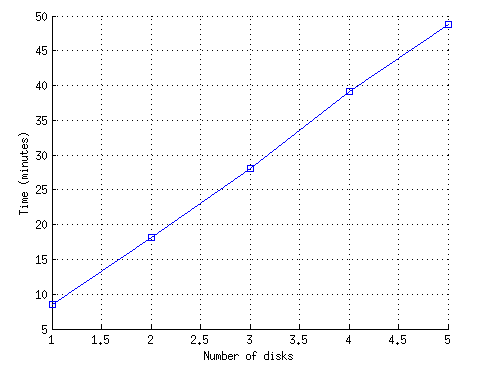
\includegraphics[width=0.65\textwidth]{logic1}
\end{center}
  \caption{Time results for complete erasure by first strategy}
  \label{fig:logic1}
\end{figure}

\newpage

%\subsection{Second strategy}
During testing erasure with second strategy we got the results presented in the Table \ref{tbl:tbl_logic2}. 


\begin{table}[h!]
  \caption{Results for complete erasure by second strategy}
  \begin{center}
  \begin{tabularx}{\textwidth}{|p{0.1\linewidth}|p{0.2\linewidth}|X|X|X|X|}
    \hline
    Disks & Capacity & Time & Average time/disk & Average speed
    \\ \hline
    1 & 18.2 GB & 10 min 54 sec & 10 min 54 sec & 27.8 MB/s \\ \hline    
    2 & 36.4 GB & 20 min 42 sec & 10 min 21 sec & 29.3 MB/s \\ \hline
    3 & 54.6 GB & 30 min 41 sec & 10 min 13 sec & 29.6 MB/s \\ \hline
    4 & 72.8 GB & 40 min 25 sec & 10 min 6 sec  & 30.0 MB/s \\ \hline
    5 & 91 GB   & 50 min 10 sec & 10 min 2 sec  & 30.2 MB/s \\ \hline
  \end{tabularx}
  \label{tbl:tbl_logic2}
  \end{center}
\end{table}
Figure \ref{fig:logic2} presents the results from the Table \ref{tbl:tbl_logic2} more clearly.
\begin{figure}[h!]
\begin{center}
  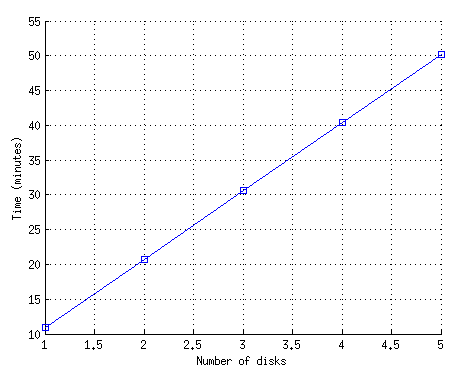
\includegraphics[width=0.65\textwidth]{logic2}
\end{center}
  \caption{Time results for complete erasure by second strategy}
  \label{fig:logic2}
\end{figure}


\newpage
%\subsection{Third strategy}
During testing erasure with third strategy we got the results presented in the Table \ref{tbl:tbl_logic3}. 


\begin{table}[h!]
  \caption{Results for complete erasure by third strategy}
  \begin{center}
  \begin{tabularx}{\textwidth}{|p{0.1\linewidth}|p{0.2\linewidth}|X|X|X|X|}
    \hline
    Disks & Capacity & Time & Average time/disk & Average speed
    \\ \hline
    1  & 18.2 GB  & 6 min 5 sec   & 6 min 5 sec  & 49.8  MB/s \\ \hline    
    2  & 36.4 GB  & 8 min 29 sec  & 4 min 15 sec & 71.5  MB/s \\ \hline
    3  & 54.6 GB  & 9 min 45 sec  & 3 min 15 sec & 93.3  MB/s \\ \hline
    4  & 72.8 GB  & 10 min 57 sec & 2 min 44 sec & 111.2 MB/s \\ \hline
    5  & 91 GB    & 10 min 57 sec & 2 min 11 sec & 138.5 MB/s \\ \hline
    6  & 109.2 GB & 10 min 57 sec & 1 min 50 sec & 166.2 MB/s \\ \hline    
    7  & 127.4 GB & 10 min 57 sec & 1 min 34 sec & 194.0 MB/s \\ \hline
    8  & 145.6 GB & 10 min 57 sec & 1 min 22 sec & 221.7 MB/s \\ \hline
    9  & 163.8 GB & 10 min 58 sec & 1 min 13 sec & 249.0 MB/s \\ \hline
    10 & 182 GB   & 10 min 57 sec & 1 min 6 sec  & 277.1 MB/s \\ \hline    
    11 & 200.2 GB & 11 min 0 sec  & 1 min 0 sec  & 303.4 MB/s \\ \hline    
    12 & 218.4 GB & 11 min 0 sec  & 55 sec       & 331.0 MB/s \\ \hline
    13 & 236.6 GB & 13 min 26 sec & 1 min 2 sec  & 293.6 MB/s \\ \hline
    14 & 254.8 GB & 13 min 28 sec & 58 sec       & 315.5 MB/s \\ \hline
  \end{tabularx}
  \label{tbl:tbl_logic3}
  \end{center}
\end{table}

\newpage
Figure \ref{fig:logic3} presents the results from the Table \ref{tbl:tbl_logic3} more clearly.

\begin{figure}[h!]
\begin{center}
  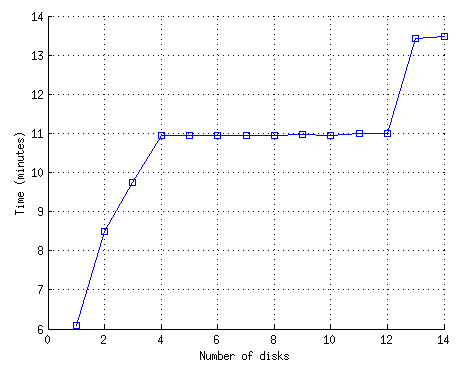
\includegraphics[width=0.65\textwidth]{logic3}
\end{center}
  \caption{Time results for complete erasure by third strategy}
  \label{fig:logic3}
\end{figure}

From the Figure \ref{fig:logic3} we can see that for disks from 4 to 12 the time of complete erasure is constant. Third strategy sends the commands parallel to several disks. That means if there is one slow disk in the task, the whole time of the erasure will be slow. Therefore, we decided to calculate the time for erasure of single disk.

\newpage
During testing erasure for single disks with third strategy we got the results presented in the Table \ref{tbl:tbl_logic3_2}. Moreover, in the Table \ref{tbl:tbl_logic3_2} we present the time of erasure for single disk during complete erasure. 

\begin{table}[h!]
  \caption{Results for erasure of single disks by third strategy}
  \begin{center}
  \begin{tabularx}{\textwidth}{|p{0.1\linewidth}|p{0.2\linewidth}|X|X|X}
    \hline
    Disks & Capacity & Time & Time during complete erasure 
    \\ \hline
    1  & 18.2 GB  & 6 min 5 sec   & 6 min 5 sec    \\ \hline    
    2  & 36.4 GB  & 9 min 39 sec  & 10 min 59 sec  \\ \hline
    3  & 54.6 GB  & 9 min 44 sec  & 9 min 43 sec   \\ \hline
    4  & 72.8 GB  & 10 min 57 sec & 10 min 59 sec  \\ \hline
    5  & 91 GB    & 10 min 55 sec & 10 min 53 sec  \\ \hline
    6  & 109.2 GB & 9 min 42 sec  & 9 min 42 sec   \\ \hline    
    7  & 127.4 GB & 6 min 37 sec  & 6 min 37 sec   \\ \hline
    8  & 145.6 GB & 8 min 29 sec  & 8 min 29 sec   \\ \hline
    9  & 163.8 GB & 6 min 38 sec  & 6 min 37 sec   \\ \hline
    10 & 182 GB   & 6 min 5 sec   & 6 min 5 sec    \\ \hline    
    11 & 200.2 GB & 10 min 13 sec & 10 min 12 sec  \\ \hline    
    12 & 218.4 GB & 9 min 51 sec  & 10 min 31 sec  \\ \hline
    13 & 236.6 GB & 9 min 55 sec  & 9 min 55 sec   \\ \hline
    14 & 254.8 GB & 6 min 6 sec   & 6 min 5 sec    \\ \hline
  \end{tabularx}
  \label{tbl:tbl_logic3_2}
  \end{center}
\end{table}

\newpage
Figure \ref{fig:compare_logic3} presents the results from the Table \ref{tbl:tbl_logic3_2} more clearly.
\begin{figure}[h!]
\begin{center}
  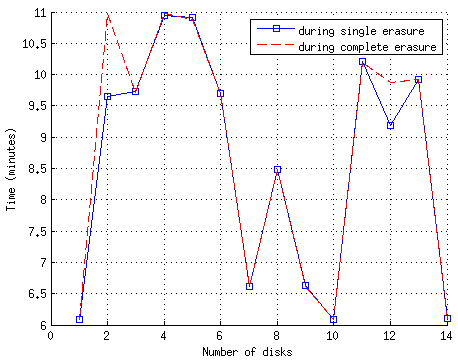
\includegraphics[width=0.65\textwidth]{compare_logic3}
\end{center}
  \caption{Time results for complete erasure by third strategy}
  \label{fig:compare_logic3}
\end{figure}

By replacing disks 4,5 and 11 we even can improve our results, which are shown on the Figure \ref{fig:better_res_WS}.
\begin{figure}[h!]
\begin{center}
  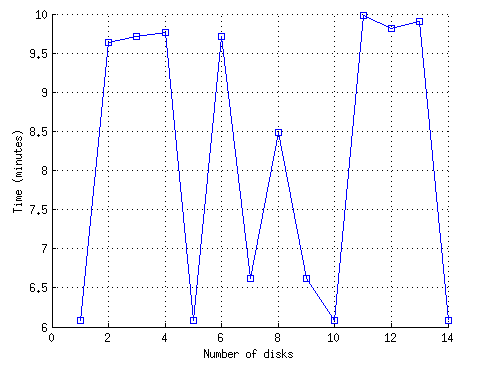
\includegraphics[width=0.65\textwidth]{better_res_WS}
\end{center}
  \caption{Time results for single erasure by third strategy}
  \label{fig:better_res_WS}
\end{figure}




\newpage
\section{Results with WRITE 10 command}
During research with WRITE SAME 10 command we understood that the parallel strategy works fine with that
controller that is why experiments with WRITE 10 command were done only with the third strategy. Several tests were done with WRITE 10 command with transfer length 256, which is not the maximum, but seems to be optimal. During testing erasure for single disks with third strategy we got the results presented in the Table \ref{tbl:tbl_write_10_01}.
\begin{table}[h!]
  \caption{Results for erasure of single disks by third strategy}
  \begin{center}
  \begin{tabularx}{\textwidth}{|p{0.1\linewidth}|p{0.2\linewidth}|X|X|X}
    \hline
    Disks & Capacity & Time & Time during complete erasure 
    \\ \hline
    1  & 18.2 GB  & 19 min 52 sec  & 53 min 43 sec (-3)\\ \hline    
    2  & 36.4 GB  & 23 min 24 sec  & 45 min 6 sec  (+4)  \\ \hline
    3  & 54.6 GB  & 23 min 28 sec  & 49 min 25 sec (+3) \\ \hline
    4  & 72.8 GB  & 24 min 43 sec  & 54 min 15 sec (0) \\ \hline
    5  & 91 GB    & 24 min 38 sec  & 57 min 39 sec (-1) \\ \hline
    6  & 109.2 GB & 23 min 28 sec  & 60 min 19 sec (+3) \\ \hline    
    7  & 127.4 GB & 20 min 27 sec  & 54 min 27 sec (+2) \\ \hline
    8  & 145.6 GB & 22 min 15 sec  & 57 min 47 sec (-3) \\ \hline
    9  & 163.8 GB & 20 min 24 sec  & 42 min 40 sec (+2) \\ \hline
    10 & 182 GB   & 19 min 50 sec  & 50 min 37 sec (-5)\\ \hline    
    11 & 200.2 GB & 24 min 1 sec   & 33 min 0 sec  (-5)\\ \hline    
    12 & 218.4 GB & 23 min 32 sec  & 35 min 10 sec (+1)\\ \hline
    13 & 236.6 GB & 23 min 39 sec  & 38 min 14 sec (-6)\\ \hline
    14 & 254.8 GB & 19 min 51 sec  & 52 min 40 sec (-5)\\ \hline
  \end{tabularx}
  \label{tbl:tbl_write_10_01}
  \end{center}
\end{table}

\newpage
Figure \ref{fig:compare_write_10_14disks} presents the results from the Table \ref{tbl:tbl_write_10_01} more clearly.

\begin{figure}[h!]
\begin{center}
  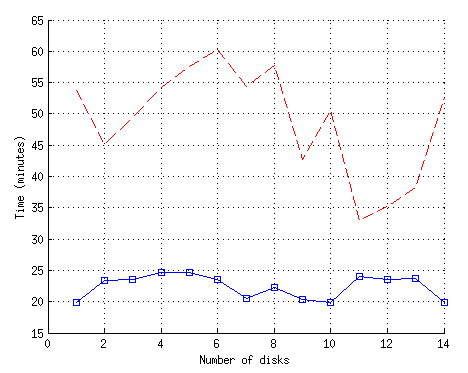
\includegraphics[width=0.65\textwidth]{compare_write_10_14disks}
\end{center}
  \caption{Time results for complete erasure by WRITE 10 command}
  \label{fig:compare_write_10_14disks}
\end{figure}


\begin{figure}[h!]
\begin{center}
  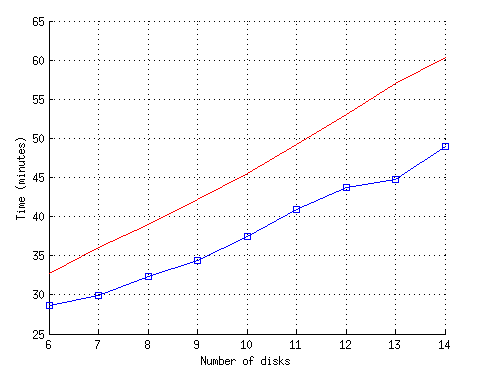
\includegraphics[width=0.65\textwidth]{aver_compl_6-14}
\end{center}
  \caption{Time results for average erasure and complete erasure}
  \label{fig:aver_compl_6-14}
\end{figure}

\newpage
Figure \ref{fig:diff_transfer_length_diskF} presents the time results for the disk 1 depending on the different transfer length.

\begin{figure}[h!]
\begin{center}
  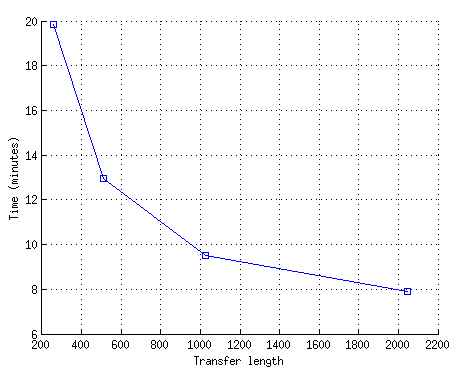
\includegraphics[width=0.65\textwidth]{diff_transfer_length_diskF}
\end{center}
  \caption{Time results for the disk 1}
  \label{fig:diff_transfer_length_diskF}
\end{figure}


\begin{figure}[h!]
\begin{center}
  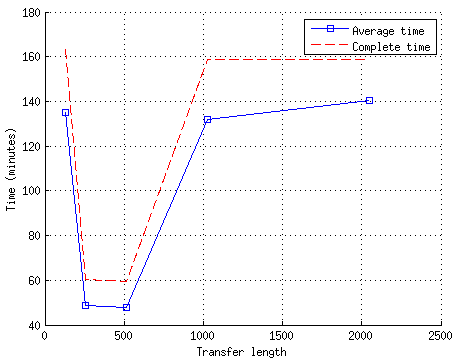
\includegraphics[width=0.65\textwidth]{diff_length_14disks}
\end{center}
  \caption{Time results for average erasure and complete erasure depending on the transfer length}
  \label{fig:diff_length_14disks}
\end{figure}


\newpage
Figure \ref{fig:comp_256_512length} presents the time results of complete erasure with transfer length 256 and 512.
\begin{figure}[h!]
\begin{center}
  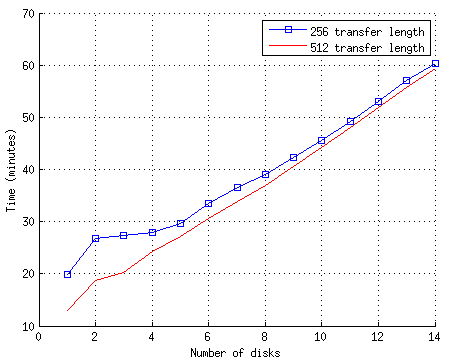
\includegraphics[width=0.65\textwidth]{comp_256_512length}
\end{center}
  \caption{Results for complete erasure depending on the transfer length}
  \label{fig:comp_256_512length}
\end{figure}

%On the Figure \ref{fig:comp_disk_repl_W10} we can notice the differences between the times for the erasure after replacement some of the disks.
\begin{figure}[h!]
\begin{center}
  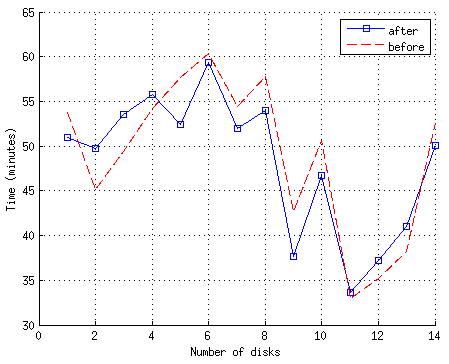
\includegraphics[width=0.65\textwidth]{comp_disk_repl_W10}
\end{center}
  \caption{Results after replacement of the disks 4,5 and 11.}
  \label{fig:comp_disk_repl_W10}
\end{figure}


\newpage
Figure \ref{fig:comp_256_best_length} presents the time results of theoretical optimal complete erasure in comparison with results with transfer length 256.
\begin{figure}[h!]
\begin{center}
  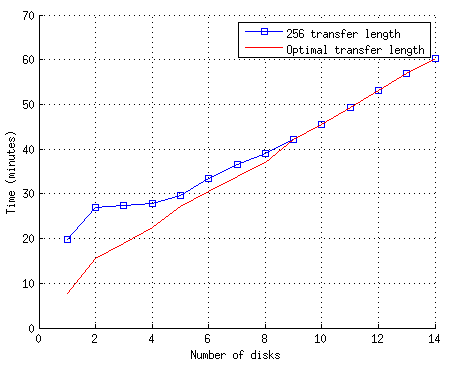
\includegraphics[width=0.65\textwidth]{comp_256_best_length}
\end{center}
  \caption{Results for complete erasure depending on the transfer length}
  \label{fig:comp_256_best_length}
\end{figure}

\begin{figure}[h!]
\begin{center}
  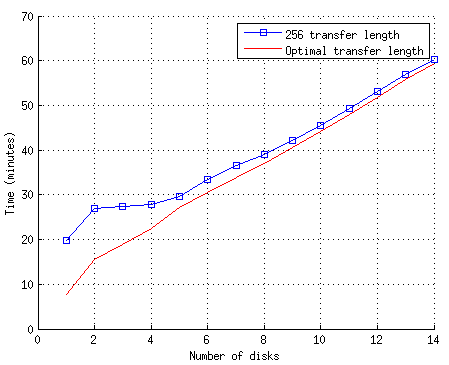
\includegraphics[width=0.65\textwidth]{comp_256_best2_length}
\end{center}
  \caption{Results for practical optimal erasure}
  \label{fig:comp_256_best2_length}
\end{figure}



\newpage
\section{Analysis of the results}

After testing with WRITE SAME 10 command we can notice that the second strategy is working slower than the first one, which is obvious because it needs to change the devices quite often. The third strategy works without any problems, but the results of several disks are quite different, which gives an idea that we did not consider all the parameters or it depends just on the hardware.

We can see from the Figures \ref{fig:logic1} and \ref{fig:logic2} that the time of first and second strategies is increasing linearly. We could not say the same about the third strategy because the disks have different speed or some other parameters disturb disk work on the maximum speed. Figure \ref{fig:compare_logic3} shows that the difference is very low between the times of erasure for single disk and for single disk during complete erasure. That means that the bus is not a bottleneck in the situation, when we send WRITE SAME 10 command and 14 disks are connected to the controller, and only rotation speed of the disks is a limiting factor. This fact is proved one more time by the Figure \ref{fig:better_res_WS}, where we show the results of erasure time for single disk during complete erasure after replacement of 3 slow disks. The results shows that the time of complete erasure decreased from 11 to 10 minutes. But still it is strange that the difference of the time of erasure for several disks can be even 4 minutes, which is almost half time of the complete erasure, but the disk parameters are completely the same.

The testing results do not depend on the application running and the erasure time is not divided randomly to different disks. Table \ref{tbl:tbl_write_10_01} proved this fact by results from the same test running several times, which gave the whole difference with -13 seconds for erasure of 14 disks by WRITE 10 command. That means that even for erasure of the fastest disk 13 seconds will take only 0.01 of whole erasure. That is why we could ignore this difference. 

We can notice that during complete erasure by WRITE SAME 10 command disks 2, 4 and 5 showed the worst time. In the same time during complete erasure by WRITE 10 command disks 6 and 8 showed the worst time. That gives an idea that there are some other parameters that also depending on the time of erasure. Moreover, Figure \ref{fig:comp_disk_repl_W10} shows how changes the results after replacement disks 4, 5 and 11. We can conclude that time for complete erasure decreased for 1 minute and the same disks show the maximum and minimum times. It is also strange that during single erasure by WRITE 10 command disks 1 and 14 were the fastest and during complete erasure their results are very closed to very slow ones.

Figures \ref{fig:diff_transfer_length_diskF} and \ref{fig:diff_length_14disks} show the results of testing different transfer length, which is one of the parameters that we can influence. To summarize these results we can say that for 14 disks transfer length 256 is definitely the optimal value, but it is not correct for 1 disk. Using the value 2048 we could erase one disk much faster. That means that the load balancing application could help with analysis, which transfer length to take, for making the erasure faster.